\documentclass[12pt]{article}

% Packages
\usepackage{graphicx}
\usepackage{listings}
\usepackage{amsmath}
\usepackage{hyperref}
\usepackage{pdfpages}
\usepackage{float}

% Document Metadata
\title{Computer Vision Project 2 Report}
\author{
    Bibek Poudel \\ Omar Mostafa \\ 
    \texttt{bp2376@nyu.edu} \\ \texttt{omm@nyu.edu}
}
\date{\today}

\begin{document}

% Title Page
\maketitle

% Section 1: Instructions to Run the Program
\section*{1. Instructions to Run the Program}

\subsection*{1.1 Compilation Instructions}
Navigate to the directory containing the source code and use the following command to compile the program:
\begin{verbatim}
python3 main.py
\end{verbatim}

\subsection*{1.2 Execution Instructions}
Compilation and execution of the program can be done using the same command:
\begin{verbatim}
python3 main.py
\end{verbatim}

% Section 2: Parameters Used for Test Images
\section*{2. Parameters Used for Test Images}

\subsection*{2.1 Test Image Pair 1: Ball}
\begin{itemize}
    \item $W$: [value]
    \item $T$: [value]
    \item $\kappa$: [value]
    \item $S$: [value]
    \item Gaussian Filtering: Yes/No
    \begin{itemize}
        \item $\sigma$: [value]
        \item Window Size: [value]
    \end{itemize}
\end{itemize}

\subsubsection*{2.1.1 Output Images}
\begin{figure}[H]
    \centering
    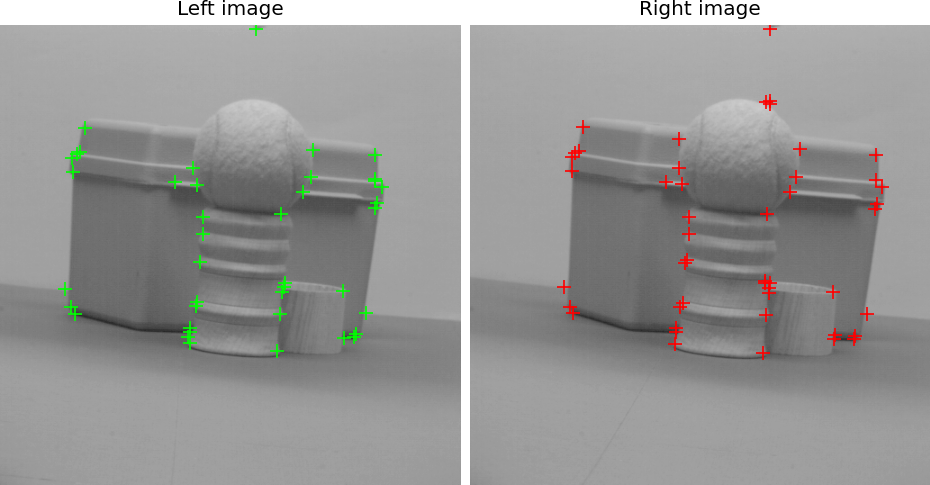
\includegraphics[width=0.8\textwidth]{stereo-imaging-harris/examples/ball/ball_corners.png}
    \caption{Ball Corners}
\end{figure}
\begin{figure}[H]
    \centering
    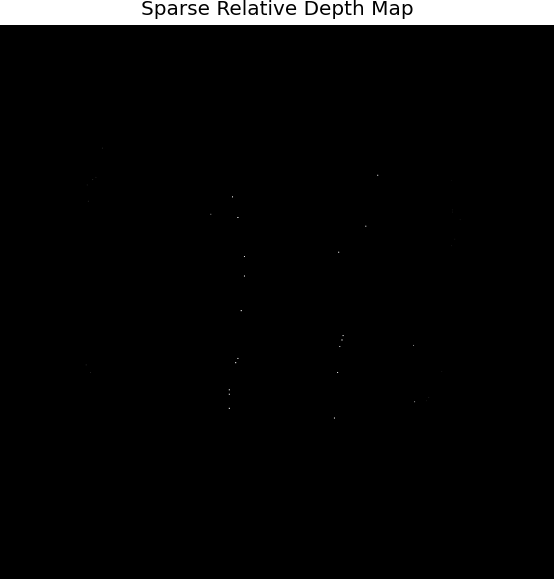
\includegraphics[width=0.8\textwidth]{stereo-imaging-harris/examples/ball/ball_sparse_depth_map.png}
    \caption{Ball Sparse Depth Map}
\end{figure}
\begin{figure}[H]
    \centering
    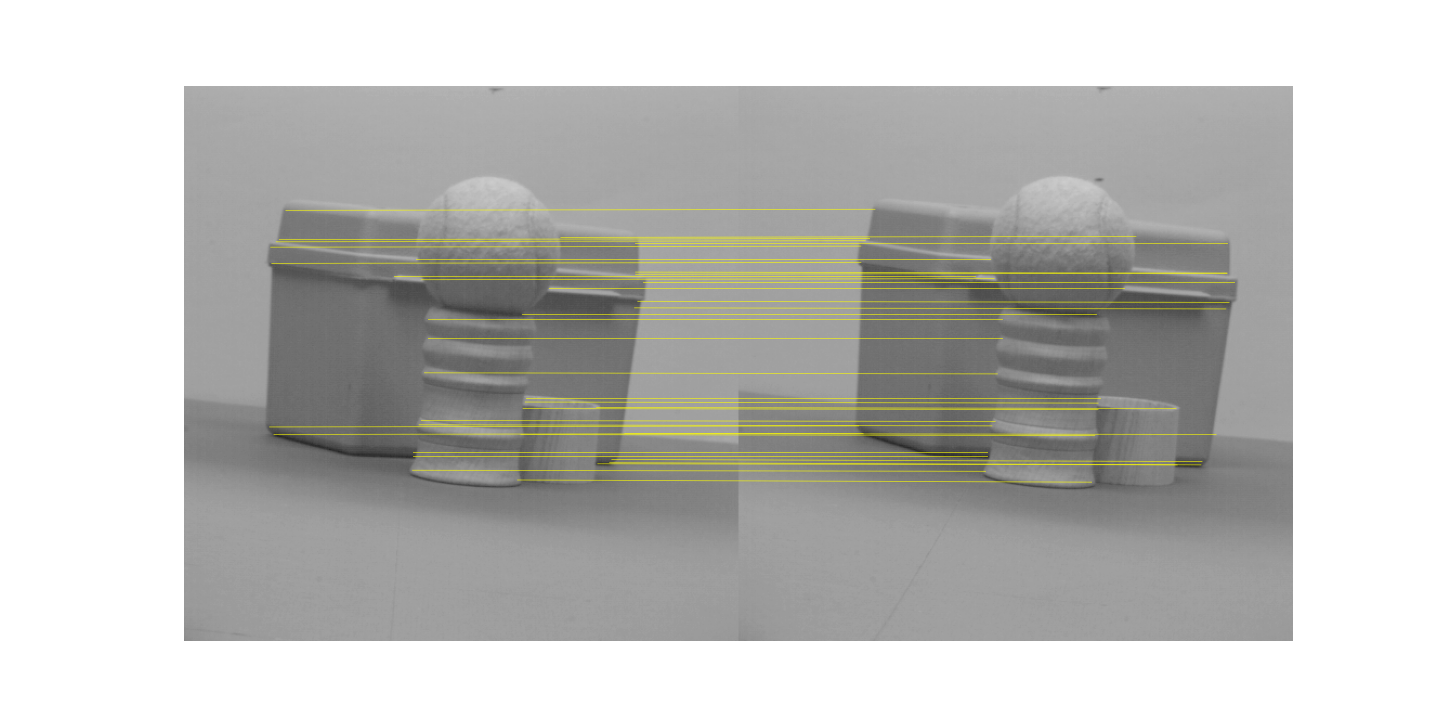
\includegraphics[width=0.8\textwidth]{stereo-imaging-harris/examples/ball/matching_ball.png}
    \caption{Ball Sparse Depth Map}
\end{figure}

\subsection*{2.2 Test Image Pair 2: Moebius}
\begin{itemize}
    \item $W$: [value]
    \item $T$: [value]
    \item $\kappa$: [value]
    \item $S$: [value]
    \item Gaussian Filtering: Yes/No
    \begin{itemize}
        \item $\sigma$: [value]
        \item Window Size: [value]
    \end{itemize}
\end{itemize}

\subsubsection*{2.2.1 Output Images}
\begin{figure}[H]
    \centering
    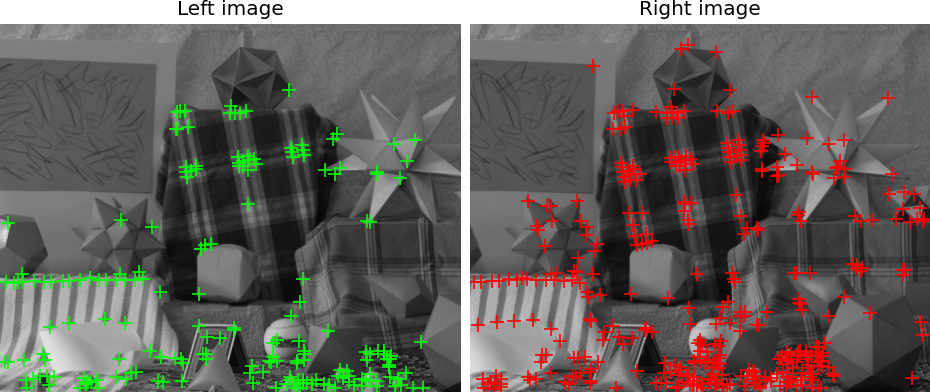
\includegraphics[width=0.8\textwidth]{stereo-imaging-harris/examples/moebius/moebius_corners.png}
    \caption{Moebius Corners}
\end{figure}
\begin{figure}[H]
    \centering
    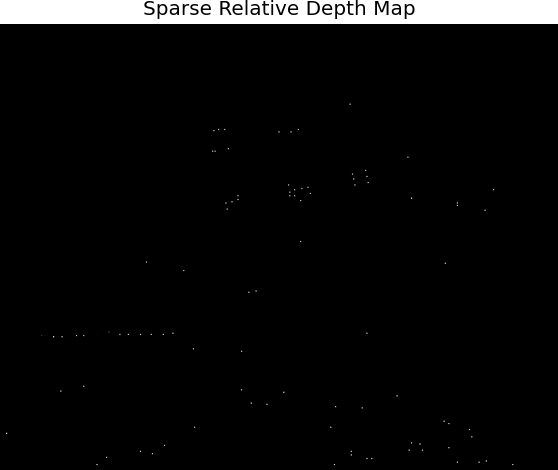
\includegraphics[width=0.8\textwidth]{stereo-imaging-harris/examples/moebius/moebius_sparse_depth_map.png}
    \caption{Moebius Sparse Depth Map}
\end{figure}
\begin{figure}[H]
    \centering
    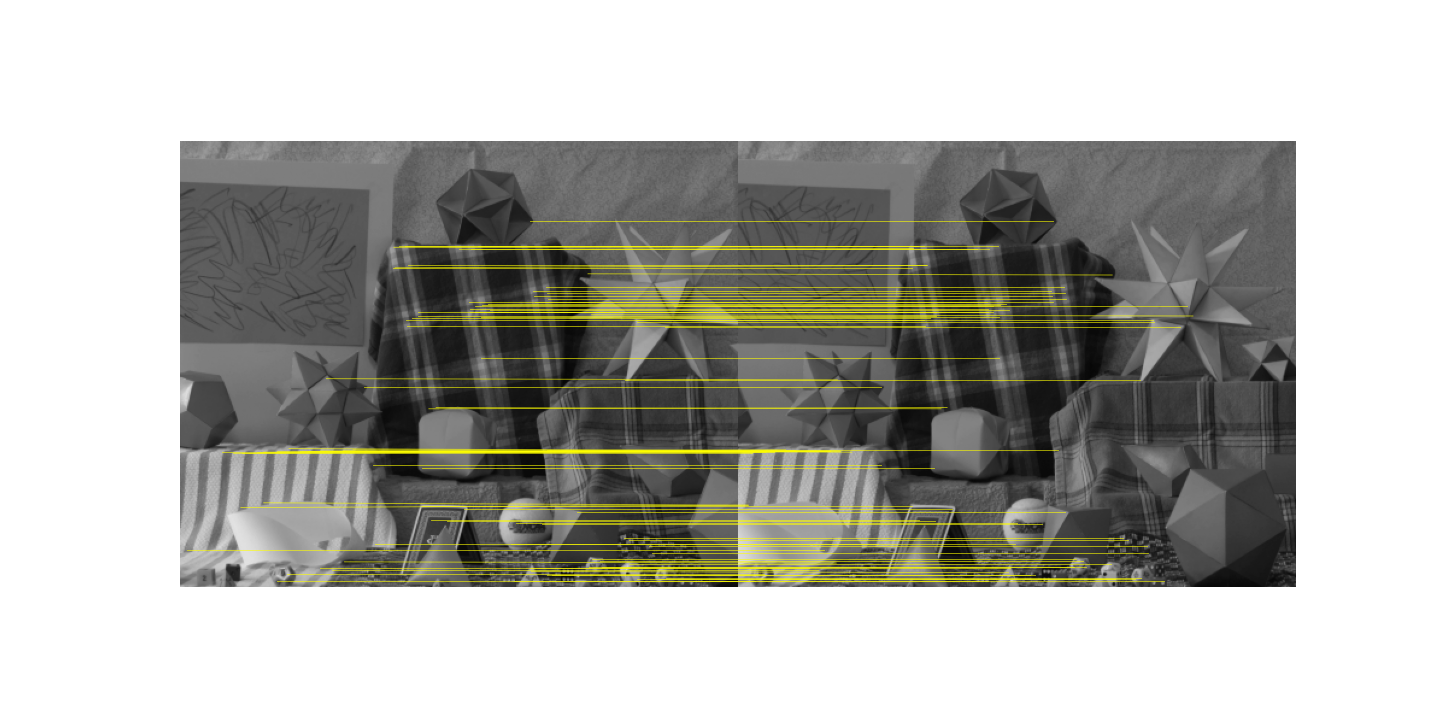
\includegraphics[width=0.8\textwidth]{stereo-imaging-harris/examples/moebius/moebous_matching.png}
    \caption{Outdoor Sparse Depth Map}
\end{figure}

\subsection*{2.3 Test Image Pair 3: Outdoor}
\begin{itemize}
    \item $W$: [value]
    \item $T$: [value]
    \item $\kappa$: [value]
    \item $S$: [value]
    \item Gaussian Filtering: Yes/No
    \begin{itemize}
        \item $\sigma$: [value]
        \item Window Size: [value]
    \end{itemize}
\end{itemize}

\subsubsection*{2.3.1 Output Images}
\begin{figure}[H]
    \centering
    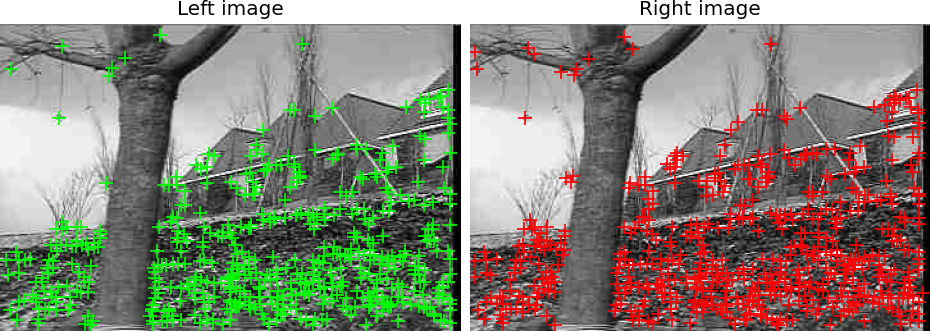
\includegraphics[width=0.8\textwidth]{stereo-imaging-harris/examples/outdoor/outdoor_corners.png}
    \caption{Outdoor Corners}
\end{figure}
\begin{figure}[H]
    \centering
    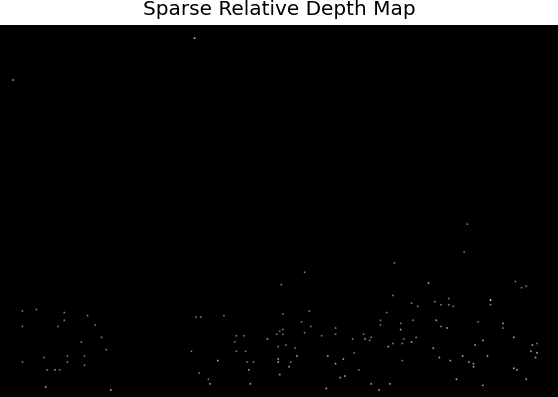
\includegraphics[width=0.8\textwidth]{stereo-imaging-harris/examples/outdoor/outdoor_sparse_depth_map.png}
    \caption{Outdoor Sparse Depth Map}
\end{figure}
\begin{figure}[H]
    \centering
    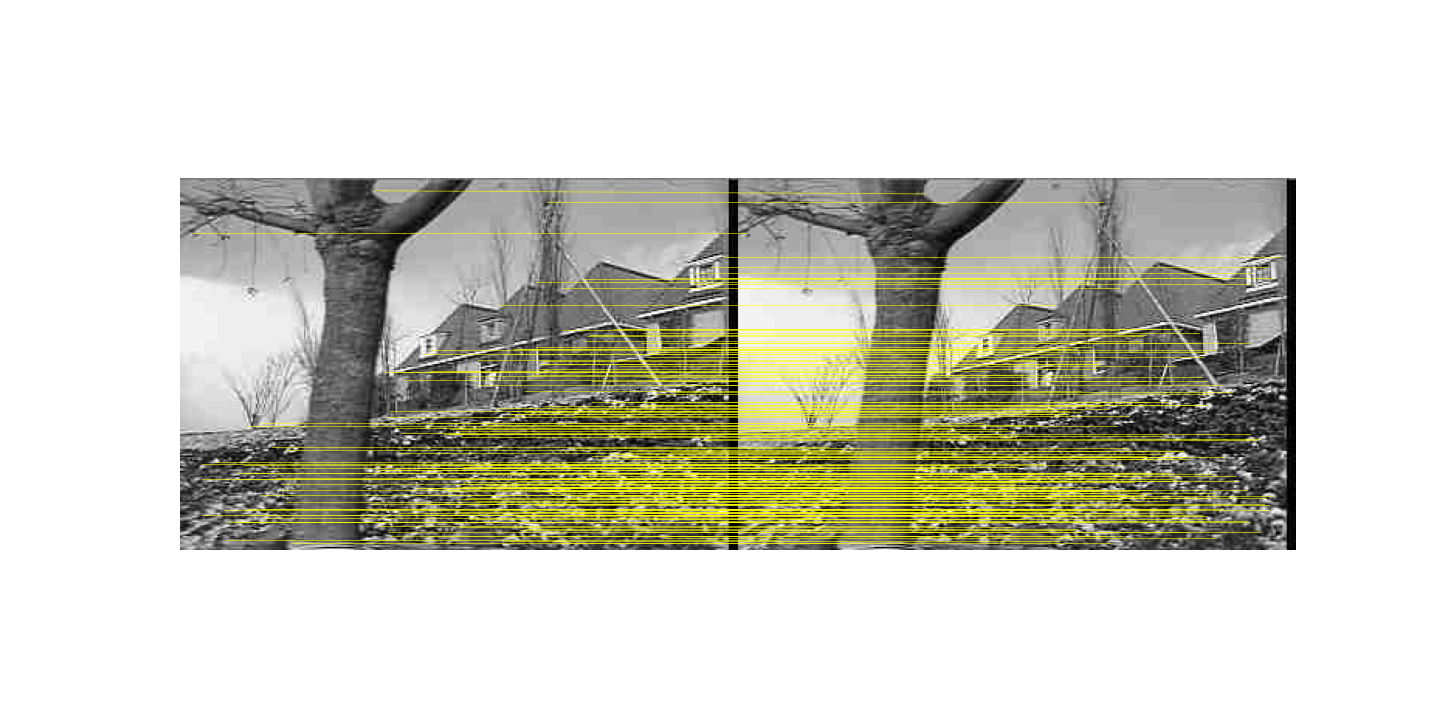
\includegraphics[width=0.8\textwidth]{stereo-imaging-harris/examples/outdoor/outdoor_matching.png}
    \caption{Outdoor Sparse Depth Map}
\end{figure}

% Include Source Code
\includepdf[pages=-]{./Source_code.pdf}

\end{document}